\subsection{Construction and Audit Details}
\label{app:benchmark-construction}

\paragraph{Design principles.}
\evolvingworldbench{} follows four principles: temporal continuity, past-only observability,
physical executability, and controlled dynamics. Examples are sampled from
persistent scene histories rather than independent placements. Public memories
contain only evidence available to the robot by the query time. Candidate states
must allow collision-free placements and reachable, visibility-checked inspection
viewpoints. Paired worlds hold the scene, target, query, and marginal placement
factors fixed while varying the hidden transition mechanism. These
controls separate predictive reasoning from scene frequency, route geometry,
and privileged simulator access.

\paragraph{Source alignment and accounting.}
Source records constrain the generator rather than serve as episode templates.
We distinguish raw source rows or sequences ($N_{\rm raw}$), records after
source-specific normalization ($N_{\rm std}$), distinct normalized records
referenced by at least one retained generation rule ($N_{\rm used}$), and total
rule references, including reuse ($N_{\rm ref}$).
Table~\ref{tab:source-accounting} reports counts from the audited consumption
manifests. This accounting prevents reuse from inflating the reported number of
independent source observations.

\begin{wraptable}{r}{0.45\linewidth}
\vspace{-0.8\baselineskip}
\caption{Audited source contributions.}
\label{tab:source-accounting}
\centering
\scriptsize
\setlength{\tabcolsep}{1.25pt}
\begin{tabular}{lrrrr}
\toprule
\textbf{Source} & $\mathbf{N_{\rm raw}}$ & $\mathbf{N_{\rm std}}$ & $\mathbf{N_{\rm used}}$ & $\mathbf{N_{\rm ref}}$ \\
\midrule
CASAS Aruba & 1,602,820 & 20,252 & 428 & 480 \\
ARAS & 5,184,000 & 5,08 & 312 & 360 \\
HD-EPIC & 59,454 & 10,786 & 742 & 864 \\
ParaHome & 212 seq. & 860 & 186 & 216 \\
OPPORTUNITY & 869,387 & 2,551 & 318 & 372 \\
HOMER+ (sim.) & 65 seq. & 1,991 & 356 & 420 \\
\bottomrule
\end{tabular}
\end{wraptable}


Raw records are sensor rows for CASAS, ARAS, and OPPORTUNITY, annotation rows
for HD-EPIC, and sequences for ParaHome and HOMER+. CASAS events are mapped to
the room ontology and split into sessions when inactivity gaps exceed 900 seconds;
the resulting occupancy, time-of-day, and weekday statistics parameterize
household schedules. ARAS and OPPORTUNITY sensor streams are segmented into
activity intervals and normalized to the shared activity, room, and object
vocabularies to provide complementary statistics on activity compatibility and
temporal context. HD-EPIC narration verbs and nouns are mapped through canonical
action and object aliases to estimate object--action frequencies, without
assigning HSSD destinations. ParaHome annotations and object transforms provide
displacement and transition-timing evidence. HOMER+ remains explicitly marked
as simulated and contributes only long-horizon activity order and terminal-state
priors, not independent human observations or test-time model inputs.

\paragraph{Mapping rules and measured parameters.}
All adapters produce records in a common schema containing time, activity, actor
context, object category, source state, destination state, and provenance. The
measured quantities are CASAS occupancy timing, ARAS/OPPORTUNITY activity context,
HD-EPIC action--object frequencies, ParaHome displacement and transition timing,
and HOMER+ simulated order priors. Legal receptacles, reachable
viewpoints, and collision-free placements are derived from HSSD geometry.
Category-to-receptacle allowlists, affordance constraints, stochastic exception
rates, paired static/routine/random interventions, the 90-day horizon, and query
sampling are benchmark-authored and labeled as such. No source trajectory is
copied verbatim, and reuse does not count as additional independent human
observations. The final manifest spans 54 scenes and 4,860 scene-days and
contains approximately 239.19k dynamic state changes and 803.68k task instances
after audits of physical validity, observability, and leakage.

\paragraph{Household generation and behavioral checks.}
For each HSSD scene \citep{khanna2024hssd}, resident schedules, room preferences,
orderliness, object ownership, and placement habits are fixed at the household
level. Activities, resident region trajectories, and object transitions are
generated jointly in chronological order over multi-day histories. Stochastic
events, delayed returns, and exceptions prevent the histories from becoming
deterministic. Household profiles, transition rules, and task templates generate
executable N1--N5, VLN, and EQA episodes. Every relocation is attributed to an activity,
resident transition, object lifecycle event, or tidying event. Personal objects
alternate between placed and carried states with owner-specific return habits;
irregular objects use affordance-valid destinations without temporal or
actor-specific predictability. Audits check that personal objects do not simply
follow their owners and that actor or activity identity does not predict
destinations for irregular objects beyond what can be predicted from affordances
alone. The audited configuration yields 42.6 region transitions per resident-day,
6.56 relocations per personal object-day, 52.6\% within-region relocations, and
zero terminal collisions.

The realized transition density in \cref{fig:routine-random-heatmaps} provides a
direct check of the paired-world intervention. Routine worlds retain repeatable,
activity-linked time bands, whereas random worlds spread changes across the day
while matching the marginal movement process. This control removes predictable
temporal phase without changing the 90-day horizon or scene setup.
The ``Change rate'' color scale shows the mean number of object relocations per
scene-day in each one-hour time-of-day bin.

\begin{figure}[!t]
    \centering
    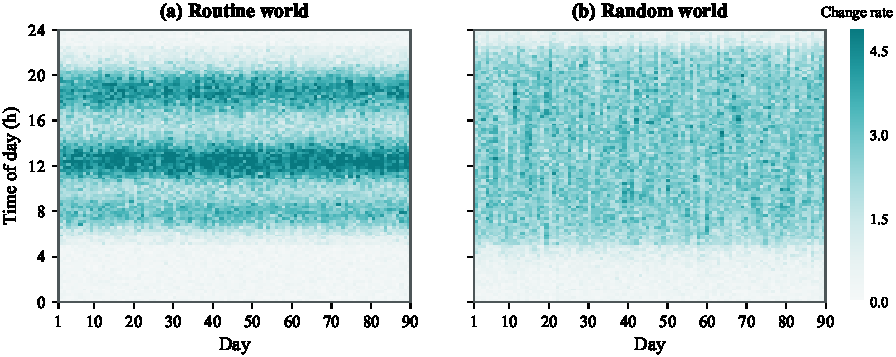
\includegraphics[width=0.94\linewidth]{figures/routine_vs_random_temporal_heatmaps.pdf}
    \caption{Temporal change density in paired routine and random worlds.}
    \label{fig:routine-random-heatmaps}
\end{figure}

\subsection{Human Review Protocol}
\label{app:human-review}

Every retained benchmark episode passes a two-stage human quality-control
process. Five trained researchers perform the primary annotation using a
structured checklist, and one supervising researcher conducts the final audit.
For each object transition, reviewers verify identity continuity, physical
validity and reachability of the destination, collision-free placement, and consistency with the
scene geometry and visibility model. They check that the transition time lies
between the relevant observations and does not expose future information. They
also record whether the reason for relocation is compatible with the attributed
activity, actor context, object affordance, or household routine. A destination may be
temporarily unobserved by the agent, as required by the benchmark, but it
must be feasible, lie within the navigable scene, and remain undisclosed in the
public history. Reviewers also check that state changes, returns, and
negative evidence are temporally ordered and semantically consistent.

Tasks are reviewed for target--episode correspondence, referent clarity,
executability, and research relevance. The target category or instance must be
instantiated in the private world state (or explicitly belong to a valid
not-found track), candidate states and viewpoints must be reachable, and the
action budget must permit a meaningful search. Language goals must identify the
intended object without answer-correlated names or future-state hints. Reviewers
check that each task probes the setting studied here, including stale
observations, hidden evolution, predictive belief, or visibility-aware evidence
updates, rather than reducing to static or trivially solvable navigation.
Reviewers accept, request revisions to, or reject each case. Disagreements are
resolved by majority vote; the supervisor adjudicates unresolved or high-risk
cases. Rejected cases are regenerated or removed, and the audit log
records the decision and reason for every retained item.

\paragraph{Candidate metadata and query sampling.}
Chronological Habitat replay records navigability, geodesic cost, camera frustum
coverage, unoccluded target fraction, and success viewpoints for each candidate.
These fields support the physical validity and visibility checks described in
\appref{app:audit}; candidates without collision-free placements and reachable
inspection viewpoints are excluded. Query times are sampled from both the natural
temporal distribution and mechanism-relevant windows, including routine stages and
intervals after a personal object is dropped. Each navigation query is augmented
with a start pose, candidate inspection viewpoints, a path budget, and frozen
success conditions. The patrol policy cannot access current object states,
resident locations, hidden activities, or generator latents. Query-time activity
and hidden transitions are retained only by the evaluator.

\paragraph{Language tasks and release documentation.}
EQA questions cover existence, location, temporal order, activity association,
count, comparison, and compositional relations over the same time-indexed
memories. Answers are evaluated against a normalized ontology, and questions
requiring future evidence are excluded. VLN replaces the object label with a language goal
whose referents and constraints are grounded in the same versioned scene history.
These task annotations support studies beyond the prediction and navigation
experiments emphasized in this paper. Across tracks, only memory representations,
current-state beliefs, and resulting decisions differ between controlled methods.
Dataset cards and audit summaries document source mappings, authored assumptions,
physical validity, candidate coverage, and leakage tests.

\paragraph{Splits and leakage checks.}
Each 90-day history uses days 0--79 for training, days 80--84 for validation,
and days 85--89 for testing. Complete temporal sequences are assigned to splits
together so that no future portion of a household day informs an earlier
decision. Held-out homes are reserved for cross-scene evaluation; paired
static/routine/random members remain in the same split. Near-duplicate queries
and transition groups are kept together when assigning splits.
Serialized releases are checked for future timestamps, private event fields,
answer-correlated filenames or indices, repeated event groups across splits,
inconsistent paired variants, invalid physics, unreachable goals, and accidental
patrol dependence on hidden state. Further details on episode-level checks and
mobility assignment appear in \appref{app:audit,app:mobility}.

\subsection{Mobility Regimes and Task Protocols}

Mobility labels are used only for stratified evaluation and are hidden from the
agent.

\begin{table}[!htbp]
\caption{Mobility regimes in \evolvingworldbench{}.}
\label{tab:mobility-regimes}
\centering
\scriptsize
\setlength{\tabcolsep}{3.5pt}
\begin{tabularx}{\linewidth}{lXXX}
\toprule
\textbf{Regime} & \textbf{Mechanism} & \textbf{Frozen signal} & \textbf{Role}\\
\midrule
Stable/rare & Infrequent events & Home/return tendency & Persistence control\\
Routine & Activity state machine & Chain-specific locations & Routine prediction\\
Personal & Placed/carried lifecycle & Owner placement habit & Long-term memory\\
Irregular & Affordance sampling & Affordance only & Uncertainty control\\
\bottomrule
\end{tabularx}
\end{table}

\begin{table}[!htbp]
\caption{Prediction and navigation protocols in \evolvingworldbench{}.}
\label{tab:tasks}
\centering
\scriptsize
\setlength{\tabcolsep}{3.5pt}
\begin{tabularx}{\linewidth}{cXXX}
\toprule
& \textbf{Task} & \textbf{Decision signal} & \textbf{Primary measure}\\
\midrule
P   & Current-state prediction & Region/receptacle belief & R@$k$ / NLL\\
N1  & Predictive navigation & Event-filtered belief & First-Inspection SR\\
N2  & Belief-guided search & Full belief + cost & Search SR / cost\\
N3  & Evidence-aware replanning & Updated posterior & Recovery SR\\
N4  & Online-dynamic navigation & Arrival-time belief & Online Recovery SR\\
N5  & Cross-scene generalization & Any protocol above & Held-out SR\\
\bottomrule
\end{tabularx}
\end{table}
\FloatBarrier
